% File SDSS2020_SampleExtendedAbstract.tex
\documentclass[11pt]{article}
\usepackage{sdss2020} % Uses Times Roman font (either newtx or times package)
\usepackage{url}
\usepackage{latexsym}
\usepackage{amsmath, amsthm, amsfonts}
\usepackage{algorithm, algorithmic}
\usepackage{graphicx}
\usepackage{adjustbox}
\usepackage{setspace}
\setstretch{0.85}
\graphicspath{{images/}}

\title{Artificial Neural Networks and Deep Learning \\
Homework 2}

\author{
  Nicola Dean \\
  10674826 \\
  {\tt nicola.dean \\
  \tt @mail.polimi.it} \\\And
  Marco Fasanella \\
  10617541 \\
  {\tt marco.fasanella \\
  \tt @mail.polimi.it} \\\And
  Raffaello Fornasiere \\
    10790353 \\
    {\tt raffaello.fornasiere \\
    \tt @mail.polimi.it} \\\And
  Christian Spano \\
  10823764 \\
  {\tt christian.spano \\
  \tt @mail.polimi.it} \\}


\date{}

\begin{document}
\maketitle


\section{Introduction}


\begin{table}[h]
\begin{center}
\begin{tabular}{|l|rl|}
\hline \bf Type of Text & \bf Font Size & \bf Style \\ \hline
paper title & 15 pt & bold \\
author names & 12 pt & bold \\
author affiliation & 12 pt & \\
the word ``Abstract'' & 12 pt & bold \\
section titles & 12 pt & bold \\
document text & 10 pt  &\\
captions & 10 pt & \\
abstract text & 10 pt & \\
bibliography & 10 pt & \\
footnotes & 9 pt & \\
\hline
\end{tabular}
\end{center}
\caption{\label{fontsizes} Sizes and styles of fonts used.}
\end{table}

\section{Example}

\begin{center}
\begin{figure}[h]
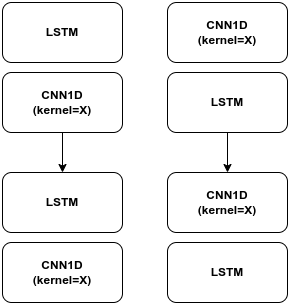
\includegraphics[width=6cm, height=4cm]{LSTMCNN}
\caption{LSTM-CNN and CNN-LSTM model schematics}
\end{figure}
\end{center}

\section{Adapt 2D models to 1D convolutions}
\subsection{InceptionNet}
\begin{center}
\begin{figure}[h]
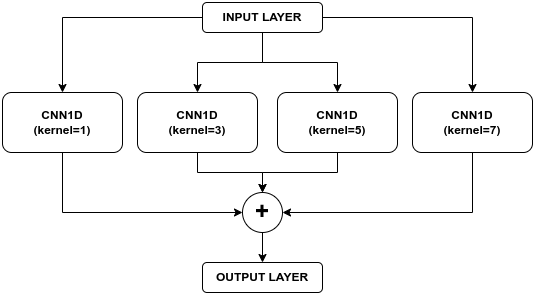
\includegraphics[width=6cm, height=4cm]{Inception}
\caption{CNN1D Inception Like Net}
\end{figure}
\end{center}

\subsection{Resnet}
\begin{figure}[h]
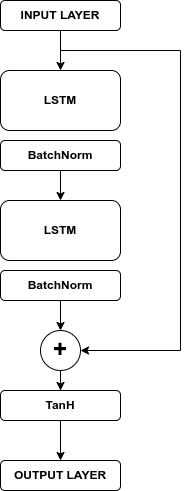
\includegraphics[width=4cm, height=8cm,angle =90]{resnet}
\caption{Resnet Like LSTM Net}
\end{figure}



\bibliographystyle{sdss2020} % Please do not change the bibliography style
\bibliography{SampleReferencesForExtendedAbstract}

\end{document}
